\documentclass{article}
\usepackage{graphicx} % Required for inserting images
\usepackage{subcaption}
\usepackage{amsfonts}
\usepackage{amsmath}
\usepackage{listings}

\bibliographystyle{plain} % We choose the "plain" reference style

\title{Multiprocessing and Parallel Systems \\ The Role of GPU in Modern Machine Learning}
\author{Marijo Simunovic}
\date{September 2023}

\begin{document}

\maketitle

\section{Introduction}
Last decade has seen a tremendous achievements in the area of Machine Learning, more specifically Deep Learning (DL) research \cite{Goodfellow2016}.
In the domain of machine learning, it is common to think about the graphic processing units (GPUs) as hardware tools that help us achieve the research goals, when in fact GPUs are integral part of this process.
The basic building block of the neural networks have been around for many years, including CNNs \cite{Lecun1998} or even decades (e.g. multilayer perceptrons) with working backpropagation solutions \cite{Rumelhart1986}.
Using the special GPU kernels to implement convolutional operators \cite{Krizhevsky2012}, Krizhevsky managed to train very deep neural networks and win ImageNet \cite{Deng2009} competition by a large margin, starting a new era in machine learning.
The other important line of research - Neural Language Processing (NLP) currently experiences upswing due to the Transformer \cite{Vaswani2017}. The Transformer managed to resolve the problems of previous Recurrent Neural Network (RNN) architectures \cite{Bahdanau2014}, \cite{Graves2013}, usually based on serialized LSTM \cite{Hochreiter1997} or GRU \cite{Cho2014} cells, utilizing the parallelizable attention mechanism, thus making it more suitable for training on multiple GPUs.

Therefore, the influence goes in both directions, research making use of powerful hardware but also hardware
determining which types of algorithms and architectures are going to survive in harsh competition of DL research environment. This also affects the way we communicate with the hardware. Initially the researchers were hacking available programming interfaces \cite{Krueger2003} to create general-purpose GPU programming (GPGPU) from which CUDA (and OpenCL) emerged, making programming on GPU much more convenient for people who aren't specialist in computer graphics.
Nowadays there are many frameworks, building on top of these low-level interfaces, which makes it lot easier to begin exploration in Deep Learning domain.
Still, it remains important to be aware of at least some of the details that are wrapped behind these high-level interfaces.

\subsection{Prototype of machine learning project}
In a typical machine learning project one designs a neural network for specific task.
The network typically consist of multiple layers where linear transformation is followed by
non-linearity (activation function) and optional pooling layers.
This kind of network can in theory approximate any function \cite{Hornik1989}.
Many variations on the theme have emerged in the last decade but that is a topic too broad for this document.
Here we give a simple example of such (convolutional) neural network, shown in Figure \ref{fig:neural_network}.

\begin{figure}[t!]
    \centering
    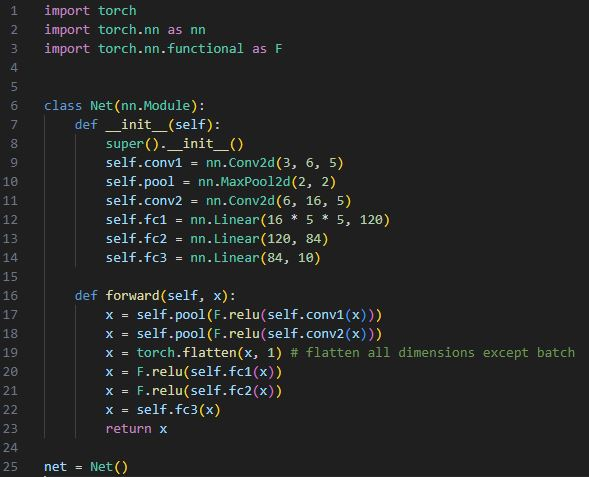
\includegraphics[width=12cm]{net.JPG}
    \caption{Simple Neural Network implemented using Pytorch Framework}
    \label{fig:neural_network}
\end{figure}

There are many high-level machine learning frameworks, PyTorch\footnote{https://pytorch.org/} and Tensorflow\footnote{https://www.tensorflow.org/} being arguably most popular ones, which enable quick design of neural networks. Unless we are defining a new type of operator (or layer)
it is sufficient to define how these basic building blocks are interconnected in terms of input and output dimensions. 
Under the hood, each layer consists of a number of parameters which we want to optimize according to the input dataset. The typical workflow is shown in code listing in Figure \ref{fig:neural_training}.
In addition to network architecture, we also need to define optimization algorithm and training criterion (i.e. loss function) that we would like to optimize. 
Data and neural network parameters are transferred to GPU and optimized in an iterative procedure, until the stopping condition has been reached.
Once the model/network has been trained, it can be used in the inference procedure in various forms.
From the code we can see that there is almost no additional work required on the side of researcher/programmer when it comes to the usage of GPU in the process.
The low-level programming typically happens in the underlying framework or even lower, in libraries which take care of nitty-gritty details of hardware \cite{Chetlur2014}, \cite{Blackford2002}.
Still, GPUs are vital part of deep learning research and it is important to understand the benefits and limitations of their usage. 

\begin{figure}[t!]
    \centering
    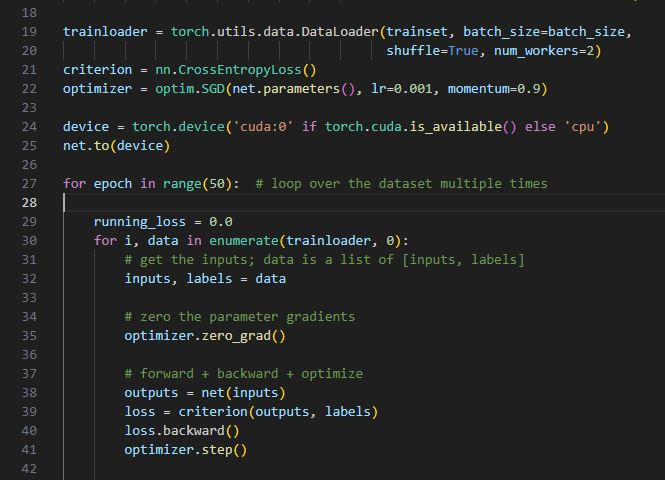
\includegraphics[width=12cm]{train.JPG}
    \caption{Standard network training setup in machine learning project}
    \label{fig:neural_training}
\end{figure}


\section{GPU Arhitecture 101}

The GPU is a processor architecture consisting of many parallel processors and of a hierarchical memory system. Unlike CPUs, which have been developed as a highly generic computing units with complicated instruction pipelines, GPUs
historically had much more limited scope of tasks. Oversimplified, the soul purpose of these devices was to
determine the color of each respective pixel on the screen with sufficient frame rate. This is achieved with shader programs working on large number of pixels in parallel. GPUs perform the task very well as the code can be organized in SIMD(Single Instruction Multiple Data)-like instructions. 
Modern GPU\footnote{I am mostly using NVIDIA terminology as this is prevalent architecture used in DL research} contains of a set of streaming multiprocesors (SMs) with a small local memory (L1 cache). Multiple SMs have access to shared memory (L2 cache). Finally, there is a larger block of slower DRAM memory (typical sizes in GBs). 
SMs employ SIMT (Single-Instruction, Multiple-Thread) architecture \footnote{In reality, there are different generations of GPU, the information here mostly refers to Volta and newer architectures} in order to be able to execute large number of threads concurrently. On a level of GPU, thread-level paralelism enables execution of different threads of code.
On a thread level, instruction level parallelism enables execution of the same instruction of different chunks of data. In contrast to CPU, there is no branch prediction or speculative execution.

Every multiprocessor manages threads in groups of 32, called \textit{warps}. All threads in a warp start at the same
instruction address. However, each of them maintains their own instruction address counter and registers and are free
to branch and execute independently. However if threads in same warp branch only the ones on the same branching path
can be executed simultaneously while other need to wait for the taken branching path to be executed completely.
Thread branching in one warp is independent of other warps.
On the level of whole GPU, multiple SMs are maintaining execution context of the wrap over entire lifetime of \textit{warp} making context switching very efficient. At every instruction cycle, warp scheduler schedules warp whose threads are ready to execute its next instruction. Each multiprocessor has set of 32-bit registers which are
shared among the warps and shared memory shared between thread blocks. For a given kernel, number of threads and blocks that can be executed on a single SM depends on their memory requirements. If there is not enough registers or
shared memory available to process at least one block, the kernel execution will fail.


\subsection{CUDA programming model}

\begin{figure}[t!]
  \begin{subfigure}[b]{0.75\textwidth}
    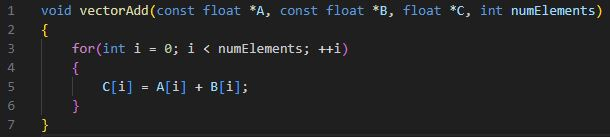
\includegraphics[width=12cm]{vector_add_c.JPG}
    \caption{CPU} \label{fig:vector_add_c}
  \end{subfigure}%
  \\
  %\hspace*{\fill}   % maximize separation between the subfigures
  \begin{subfigure}[b]{0.75\textwidth}
    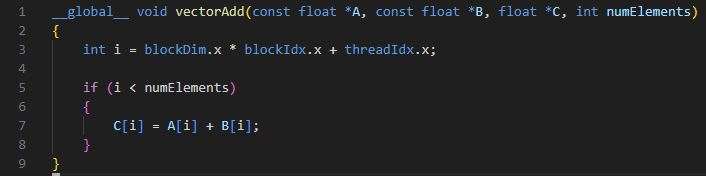
\includegraphics[width=12cm]{vector_add_cu.JPG}
    \caption{GPU} \label{fig:vector_add_cu}
  \end{subfigure}%
  

\caption{Vector Add Function implementation on different targets} \label{fig:1}
\end{figure}

CUDA (Compute Unified Device Architecture) programming model assumes existence of \textit{host} and \textit{device}
systems, each maintaining their own independent memory. The host code takes care of initialization of resources and
transfer of data. After the data is on GPU device, host schedules execution of \textit{kernel} - a block of code
implemented in CUDA programming language. Once the processing is done, host schedules retrieval of the results from device and de-allocates the resources. \\
If we squint a bit, programs written for the GPU looks quite similar to those written for the execution on CPU. 
In a typical introductory example \footnote{https://github.com/nvidia/cuda-samples}, the Figure \ref{fig:vector_add_c} shows the implementation of addition of two vectors on CPU and a same function written for NVIDIA GPU in Figure \ref{fig:vector_add_cu}.
However, user code is quite more complicated,  as visible in Figure \ref{fig:main}, for the GPU case.
Firstly, we need to allocate the data on the host and initialize the inputs.
After that, we need to allocate the resources (\textit{cudaMalloc}) on GPU and transfer the data from host (\textit{cudaMemCpy} with \textit{cudaMemcpyHostToDevice} flag).
Kernel is invoked with user specified thread block organisation 
\begin{lstlisting}[language=C]
  vectorAdd<<<blocksPerGrid,threadsPerBlock>>>
  (d_A, d_B, d_C, numElements);
\end{lstlisting}
The \textit{blocksPerGrid} and \textit{threadsPerBlock} are used to optimize the usage of GPU.
Therefore, their values are going to depend on both the problem at hand and the underlying compute capability of hardware.
After that the results are copied back to host (\textit{cudaMemCpy} with \textit{cudaMemcpyDeviceToHost} flag).
The allocated resources needs to be in the end cleaned up and device optionally reset.
In the GPU programs it is also common to have many error checks sprinkled around which we leave out for brevity.
We can see already on this simple example that the usage of GPUs can become quite involved.
This is of course justified with the increased amount of compute that GPUs provide and without which
modern Deep Learning would be hardly imaginable. 

\begin{figure}
    \centering
    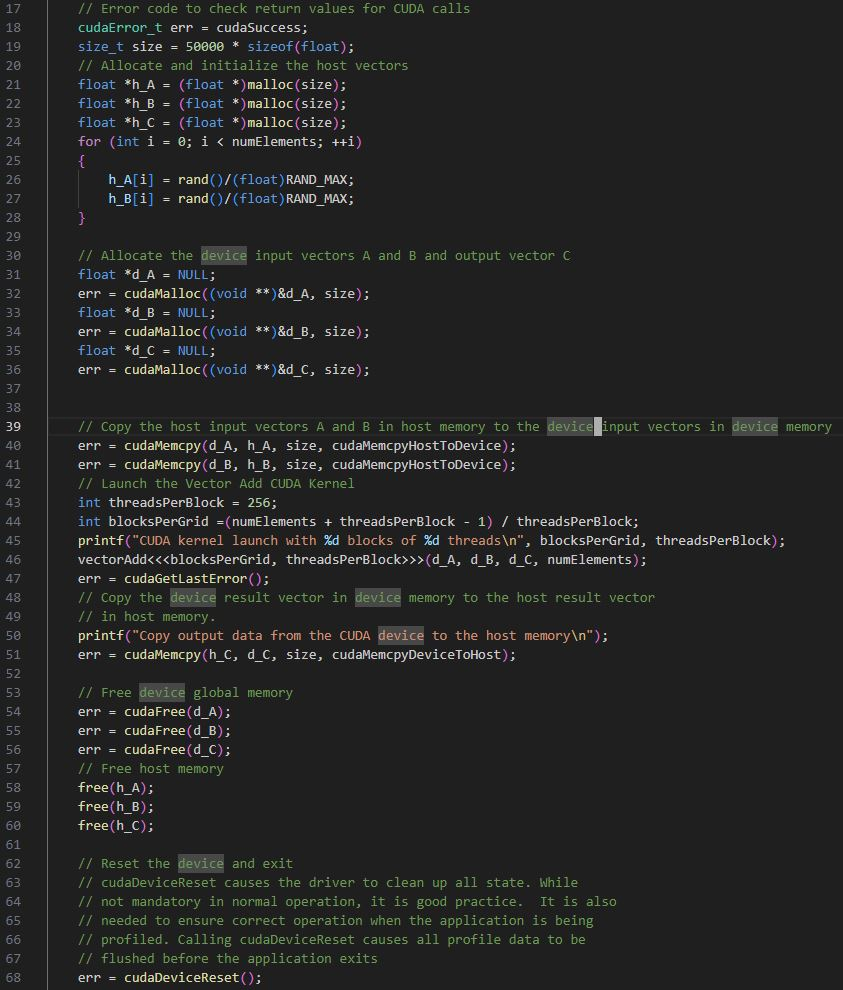
\includegraphics[width=12cm,height=18cm]{main.JPG}
    \caption{User code for the GPU vector addition kernel}
    \label{fig:main}
\end{figure}


\section{GPU from a perspective of machine learning}

\subsection{Loading the data onto the GPU}
As previously mentioned, one of the first steps in setting up the machine learning project is loading the data and moving it to the GPU.
Because large amount of data can be processed we need to ensure that sufficient amount of data is
available on the device.
One way to achieve this, often used in DL projects, is to pin the memory, changing the line 19 in Figure \ref{fig:neural_training} to:
\begin{lstlisting}[language=Python]
trainloader = torch.utils.data.DataLoader(
    trainset, batch_size=batch_size,
    shuffle=True, num_workers=2, pin_memory=True)
\end{lstlisting}
The host device's OS uses paging\footnote{https://en.wikipedia.org/wiki/Memory\_paging} to manage usage of main memory. 
The GPU cannot access data directly from pageable host memory as the memory address space could become invalid at any point.
When the data transfer occurs, the CUDA driver allocates a temporary page-locked, \textit{pinned} array of memory, copies the data to this dedicated memory area and then initiates the transfer on
the device.
However, if we use the \textit{pin\_memory} option, as in our code example, this intermediate step is skipped.
One negative side of this method is that the allocated memory is no longer available to the other processes on the host device.
The other popular method to optimize data transfers, especially during the training when the data is already available, is to batch data transfers, transferring multiple input data objects to the GPU at the same time.
\subsection{Common operators of machine learning}
Even though modern Deep Learning architectures are quite complex, they are most often consisting of blocks of common
operators which can broadly be separated in three groups:
\begin{enumerate}

\item  Elementwise operators - performed on each element of tensor independent of all other elements (e.g. ReLU operator, elementwise operation). Low number of performed compute instructions per number of bytes of data makes this operation memory-limited
\item  Reduction operators - performed over a range of elements of tensor an can produce one or more new values (e.g. SoftMax activation function, pooling layers, etc.). Similarly to elementwise operators these are usually memory-limited 
\item  Matrix multiplications - most commonly compute sum of products of two matrices/vectors (e.g. fully-connected layers, convolution operators). These can be either memory-bounded for smaller matrices or math-bounded if larger matrices are involved in operations

\end{enumerate}
\subsubsection{Convolutions as a workforce of Computer Vision architectures}
Convolutional Neural Networks  \cite{Lecun1998} are quite popular in the domain of computer vision. One of the reasons for their popularity is that the convolution operator can be quite efficiently implemented on the GPUs. This implementation is not intuitive but the result of utilizing the already existing optimized routines for general matrix multiplications (GEMM).\\
TODO: insert images\\
Convolutions are simple feature detectors, filters $F \in \mathbb{R}^{NCH_fW_f}$ acting on the input tensor $X \in \mathbb{R}^{BCHW}$. The input is batch of size $B$ with $C$ input feature maps (channels) of $H$ rows (height) and $W$ columns (width). Convolutional filter bank must have same number of input feature maps $C$. $H_f$ and $W_f$ determine the size of patch of input that the filter sees and $N$ is the number of output feature maps. The size of the output is also 4D tensor $Y \in \mathbb{R}^{BNW_oH_o}$.
First two dimensions $B$ and $N$ and determined by the batch size of the input and the number of filters $N$. Height and width dimension of the output depend on the height and width of input together with selected padding and stride choices. Padding parameter describes how much rows and columns to append to the input (when filter operates on the "edge" of the input). Striding allows skipping the rows and columns between starting rows and columns on which filters are applied. 
The single value of the output (at $b, n, w, h$ coordinate) is calculated as:
\begin{equation}
    Y[b,n,w,h] = \sum_{c=o}^{C-1}\sum_{h_f=0}^{Hf-1}\sum_{w_f=0}^{Wf-1} F[n,c,h_f,w_f] * X[b, c, ps(w), ps(h)]
\label{conv_eq}
\end{equation}
where $ps(x)$ is access function on the input depending on the selected padding and stride options.
From (\ref{conv_eq}) we can see that the convolution is in fact seven-way nested loop with three accumulation loops and four independent loops (over each dimension of output $B, N, W_o, H_o$).
\begin{figure}
    \centering
    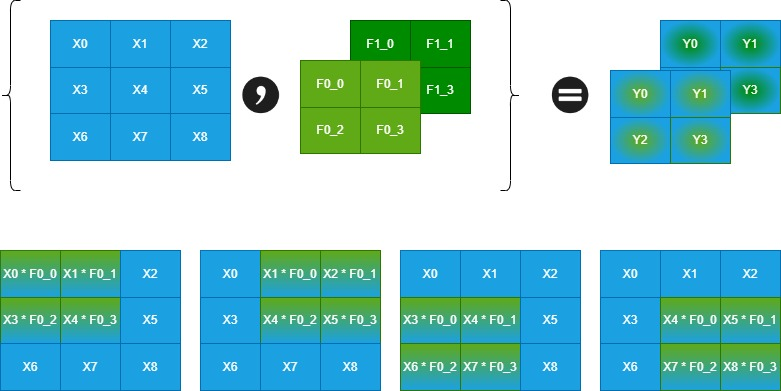
\includegraphics[scale=0.4]{ConvDiagram_Naive.jpg}
    \caption{Naive implementation of convolutional operator}
    \label{fig:conv_naive}
\end{figure}
One can easily imagine (see Figure \ref{fig:conv_naive}) the procedural implementation of this equation with nested \textit{for}-loops and the auxiliary code checking the edge conditions (padding) and hops (depending on the stride). Such code is quite natural on the CPU machine where the number of possible threads is typically small and the overhead of running multiple treads quickly overcomes the benefits of parallelism. On GPU however, parallelisam is "native" and it is
cheap to run a thread for each output value. We can avoid having many loops by mechanism of \textit{lowering}. This encompasses reorganizing the filters and input in a layout that is much more convenient for execution 
\begin{figure}
    \centering
    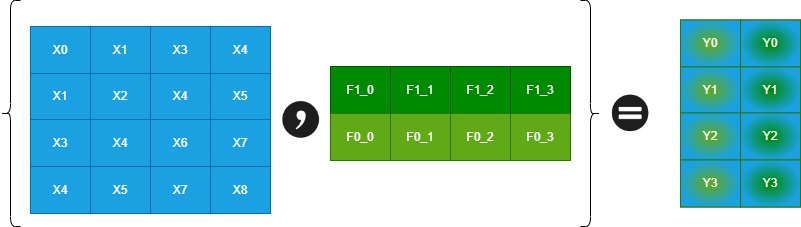
\includegraphics[scale=0.4]{ConvDiagram_Lowering.jpg}
    \caption{Implementation of convolutional operator with \textit{lowering}}
    \label{fig:conv_lowering}
\end{figure}
with optimized GEMM operations. The increased performance comes at the expense of increased memory consumption. In Figure \ref{fig:conv_lowering} we can see that for our example, input increases to 4x4 size from initial 3x3.
\subsection{Training overhead}
The goal of training in Deep Learning is to find the parameters \textbf{$\Theta$} that reduce some cost function \textbf{$J(\Theta)$}. The performance is typically measured on the entire (training) set.
In the end, we care about some performance measure $P$ on inference set, which can only be determined indirectly, using $J$ as a proxy. This is in contrast to pure (mathematical) optimization where minimizing $J$ is the actual goal. 
The cost function\footnote{supervised task} can be written \cite{Goodfellow2016} as an average over the training set:
\begin{equation}
    J(\Theta) = E_{(\textbf(x), y) \sim p_{traindata}}L(f(\textbf{x}; \Theta), y)
\end{equation}
where $L$ is per sample loss function, $f$ is predicted output with input $x$ and network parameters $\Theta$ and $y$ is the ground truth value. 
This formulation can be extended for various forms of regularization or for unsupervised learning tasks. \\
Given the dataset sizes and huge number of parameters in the neural networks, optimization over entire set in a single iteration would be quite slow. Additionally we cannot store all the parameters for the training at the same time on a GPU. In practice, we usually use only a small batch of data in a single step, i.e. using stochastic methods. \\
Special care is also given to the way how parameters are initialized \cite{Glorot2010} and there are different regularization strategies \cite{Ioffe2015}, \cite{Srivastava2014} or optimization algorithms \cite{Kingma2017} that can additionally contribute to the memory consumption.
During the training, all intermediate data (activations, weights, gradient updates) must be kept in memory.
Therefore, the "optimal" setup for each respective project will vary and requires iterative process if we aim to fully utilize underlying hardware. Even though modern GPUs like NVIDIA A100
offer large amount of memory it is still possible to run into Out-Of-Memory (OOM) issues.
Recent methods \cite{Dao2022}, \cite{Dao2023} in training are trying to overcome this issues by implementing neural networks operators in more IO-aware fashion improving the GPU utilization.

\subsection{Computational types}
\begin{figure}[t!]
    \centering
    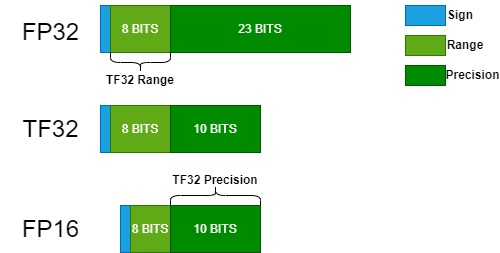
\includegraphics[width=8cm,height=4cm]{tf32.jpg}
    \caption{TF32 format range and precision structure. Adapted from  \\  https://blogs.nvidia.com/blog/2020/05/14/tensorfloat-32-precision-format/}
    \label{fig:tf32}
\end{figure}
AI computation has traditionally relied on the usage of IEEE 754 single-float precision format (FP32).
Due to the fact that floating point operations of addition and multiplication are not associative it is not possible to guarantee bitwise identical results of computations even after controlling for the sources of randomness.
In practice, this issue often surfaces when we are changing (upgrading) versions of the frameworks or GPU drivers.
This is important issue as the reproducibility is a hallmark of any scientific research.\\
Going in the other direction, reducing the precision can help speeding up the training and reduce the memory requirements.
This is the reason why the AI frameworks often support the mixed precision calculations.
When mixed precision is used, calculations start with half-precision input values and the results are then stored in higher precision, e.g. multiplying two 16-bit (FP16) matrices together and storing the answer as FP32 values).
It has been observed in practice, that neural networks often achieve same, or almost the same performance even when half-precision values are being utilized.
Modern GPU architectures offer specialized cores (Tensor Cores in case of NVIDIA GPUs) that are dedicated to this kind of computation.
These cores are especially optimized for the matrix-multiplication types of operations which are so common in Deep Learning.\\
Apart from being able to use traditional floating precision formats, these cores enable computation with new hybrid formats.
One such format is TF32 shown graphically in Figure \ref{fig:tf32}.
TF32 uses the 10bit mantissa as FP16 format which has sufficient margin for the precision requirements in AI related applications and the 8bit exponent as FP32 so it can support the same numeric range.
This combination makes TF32 a good alternative to FP32 for massive multiply and accumulate operations common in DL while achieving significant speedups at training and inference times.

\section{Inference and target hardware}



After neural network has been trained to sufficient performance, measured on the test set it can be used for inference in practical applications.
It is often the case that the inference model is not executed on the same platform as it has been trained on.
The other issue is that most of the AI frameworks are written in Python which makes it harder to use models stored in their native format.
Open Neural Network Exchange (ONNX) is an open format for machine learning models which allows the interchange of models between the frameworks and tools.
It represent the neural network in a form of a computational graph model with standardized operators and data types.
Figure \ref{fig:net_onnx} shows the ONNX representation of the neural network from Figure \ref{fig:neural_network}. 
This portable format enables optimization of the neural network for a specific inference hardware.
Most common optimizations consist of:
\begin{itemize}
    \item quantization - reducing the higher precision values of parameters to the lower precision floating point or even integer representations,
    \item layer fusion - merging multiple operations into a single one thereby reducing the number of instructions and memory transfers that need to be performed,
    \item kernel tuning - selecting the kernels (algorithms) that perform best on the target hardware.
\end{itemize}
\begin{figure}[t!]
    \centering
    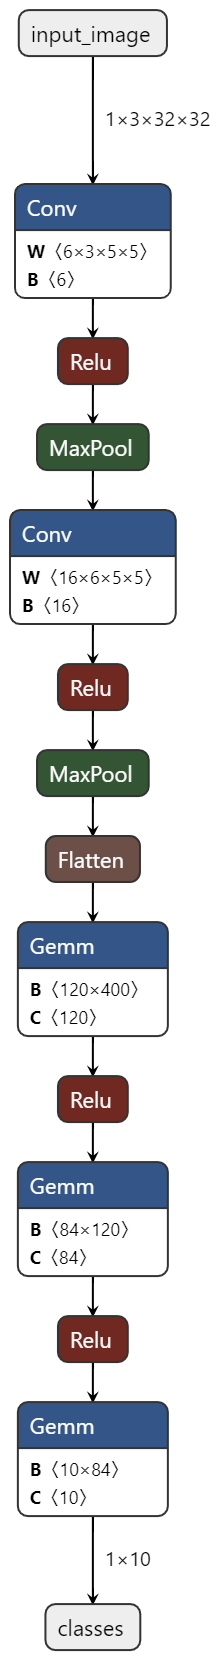
\includegraphics[height=10cm,width=2cm]{net_onnx.png}
    \caption{ONNX representation of the neural network in Figure \ref{fig:neural_network}}
    \label{fig:net_onnx}
\end{figure}
ONNX is however not a silver bullet solution.
There are multiple complications which arise when porting the model to a target architecture.
Some operators might not be supported on a given hardware.
ONNX is not that flexible and there are complications that occur if we want to allow for dynamic input dimensions or if there is a conditional logic in the network algorithm.
It is therefore necessary to take into account the specifics of target hardware into the design of neural network architectures.

\section{Conclusion}
The Deep Learning brought a new set of challenges in terms of execution of the programs. The programs executed on
GPUs are no longer only shaders and rasterizers but complicated computational graphs. This influenced the architectural design (e.g. introduction of ThreadCores) as well as the programming API (CUDA instead
of GPGPU programming).
As the sizes of modern Deep Learning architectures constantly push the limits of the available GPUs, new GPU architectures are becoming more complex.
While this makes it harder to know all the intricate details of specific architectures, it remains important to understand the opportunities and limitations given by the underlying hardware that we use.
This can often make a difference between successful and failed machine learning projects.

\bibliography{references_MPS}

\end{document}
